\documentclass{beamer}
\setbeamertemplate{navigation symbols}{}
\setbeamertemplate{caption}{\insertcaption}
\usetheme{Dresden}
\usepackage{amsmath}


\beamersetuncovermixins{\opaqueness<1>{25}}{\opaqueness<2->{15}}

\begin{document}
	\title{Stats for Data Science}  
	\author{Saumya Bhatnagar}
	\date{\today} 
	
	
\begin{frame}
\titlepage
\end{frame}

\begin{frame}\frametitle{Table of contents}\tableofcontents
\end{frame} 


\section{Glossary}
\subsection{Initial Terminologies} 
\begin{frame}
\begin{figure}
	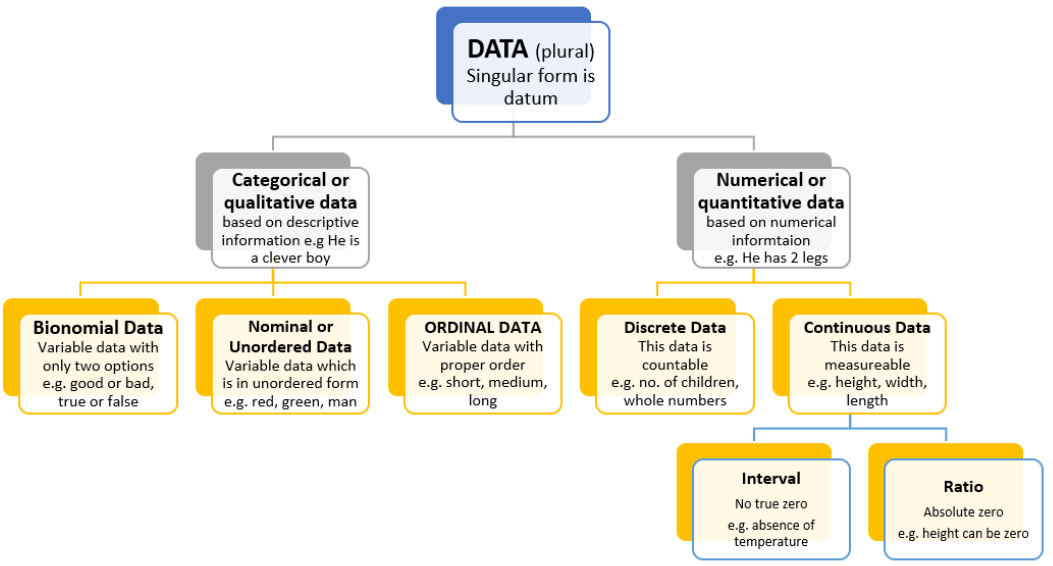
\includegraphics[scale=0.4]{Data} 
	%\caption{t-test, anova, chi-square, correlation test}
\end{figure}
\end{frame}

\begin{frame}\textbf{Types of Analysis}
\begin{itemize}
\item Qualitative Analysis/Non-Statistical Analysis gives generic information (uses text, sound and other forms of media).
\item Quantitative Analysis/Statistical Analysis: collecting and interpreting data.

\end{itemize}
\begin{figure}
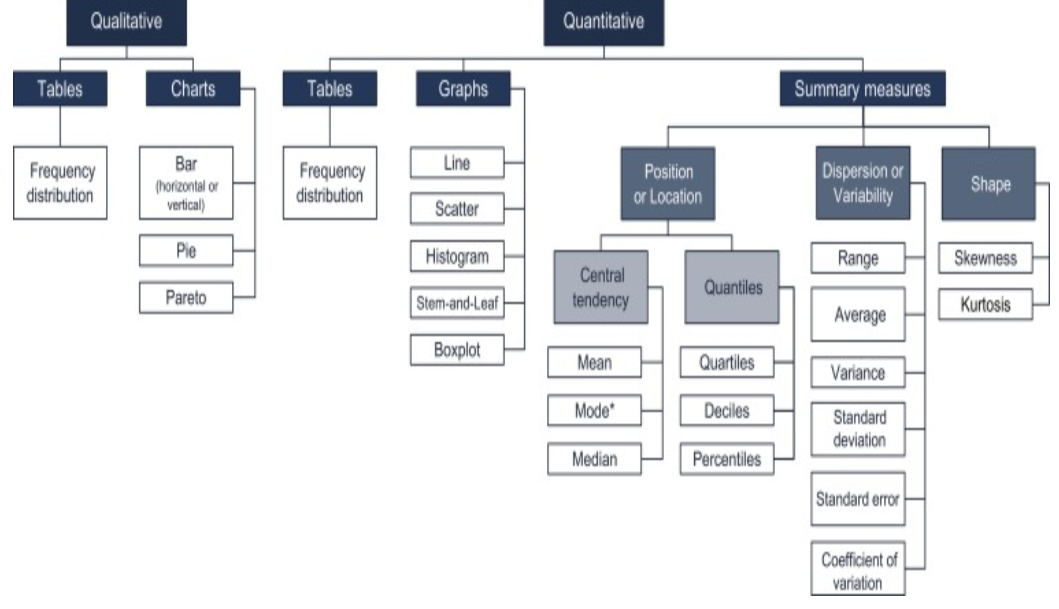
\includegraphics[scale=0.3]{QuantitativeQualitative} 
%\caption{t-test, anova, chi-square, correlation test}
\end{figure}
\end{frame}



\begin{frame}\frametitle{Types of Statistics}
\begin{itemize}
\item Descriptive Statistics: provides descriptions of the population.
\item Inferential Statistics makes inferences and predictions from sample to generalize a population. 
\end{itemize}

\begin{figure}
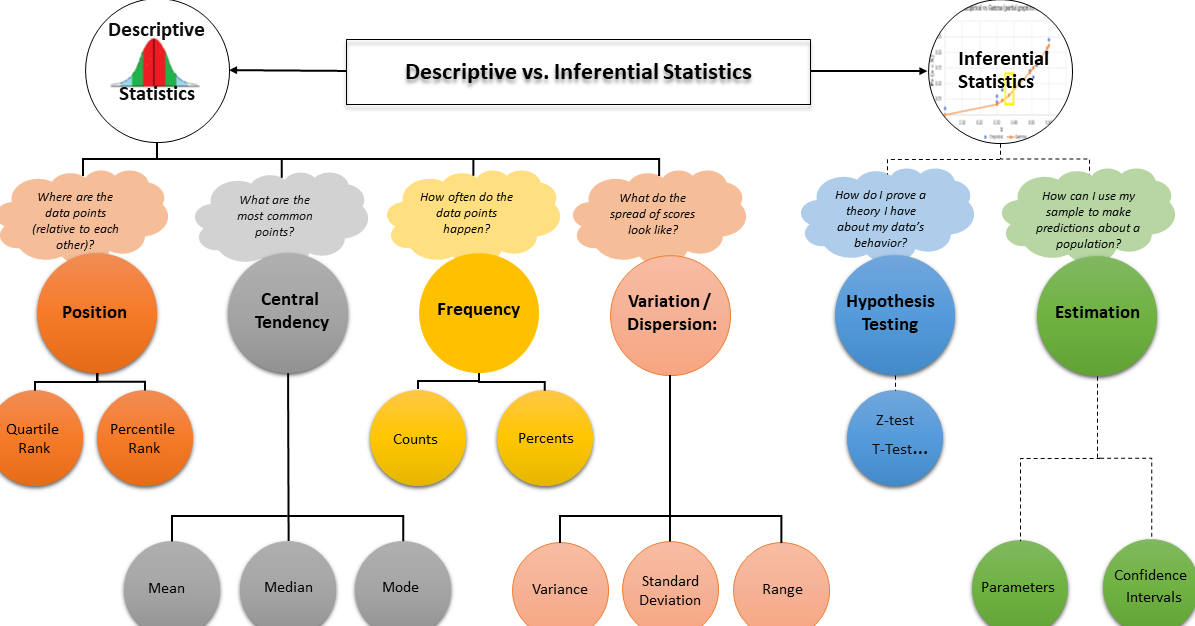
\includegraphics[scale=0.29]{DescriptiveInferential} 
%\caption{t-test, anova, chi-square, correlation test}
\end{figure}
\end{frame}

\begin{frame}[plain]
\begin{figure}%[plain]
\makebox[\linewidth]{\includegraphics[width=\paperwidth]{inferentialstats}}
\end{figure}
\end{frame}


\begin{frame}\textbf{Contingency Table and Probabilities}
\begin{figure}
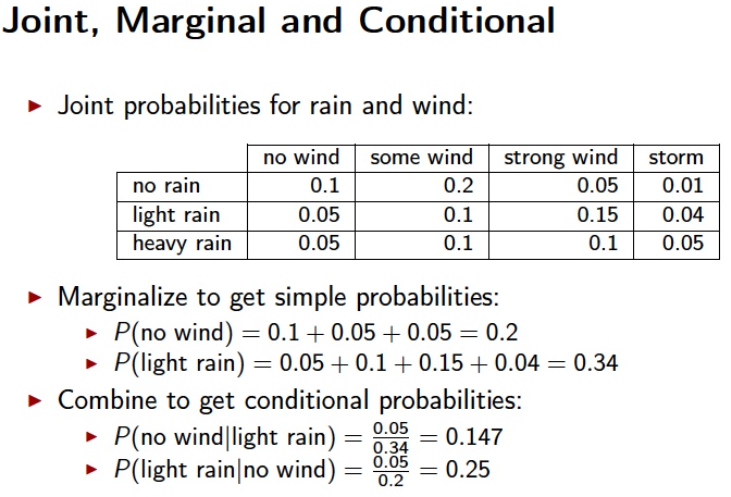
\includegraphics[scale=0.5]{JointMarginalConditional} 
%\caption{t-test, anova, chi-square, correlation test}
\end{figure}
\end{frame}



\begin{frame}\frametitle{Central Limit Theorem(CLT)}
\textbf{CLT}: as n $\uparrow$, the distribution of sample mean or sum approaches a Normal Dist\\
Law of large num \\ law of averages\\
\end{frame}


\subsection{Types of Distributions} 

\begin{frame}\frametitle{PMF, CMF, PDF, CDF}
\begin{columns}
	\begin{column}{5cm}
		\begin{itemize}
			\item<1> A PMF, “f” returns the probability of an outcome: $f(x)=P(X=x)$ 
			 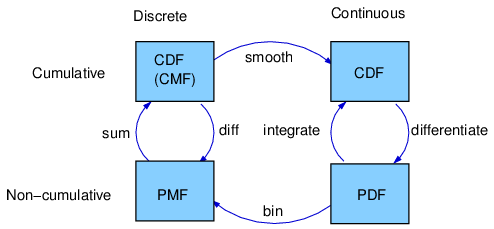
\includegraphics[scale=0.35]{CdfPdfPmf} 
			 \newline
			\item<2> Reliability function \& Hazard Function
		\end{itemize}
		\vspace{3cm} 
	\end{column}
	\begin{column}{5cm}
		\begin{overprint}		
			\includegraphics<1>[scale=0.3]{PmfCdfContinuous}
			\includegraphics<1>[scale=0.25]{pdfcdfDiscrete}
			\includegraphics<2>[scale=0.32]{cdfpdfrfhf}
		\end{overprint}
	\end{column}
\end{columns}
\end{frame}


%%%%%%%%%%%%%%%%%%%%%%%%%%%%%%%%%%%%%%%%%%%%%%%%%%%%%%%%%%%%%%%
\begin{frame}
	\begin{columns}
		\begin{column}{0.69\paperwidth}
			\begin{figure}
				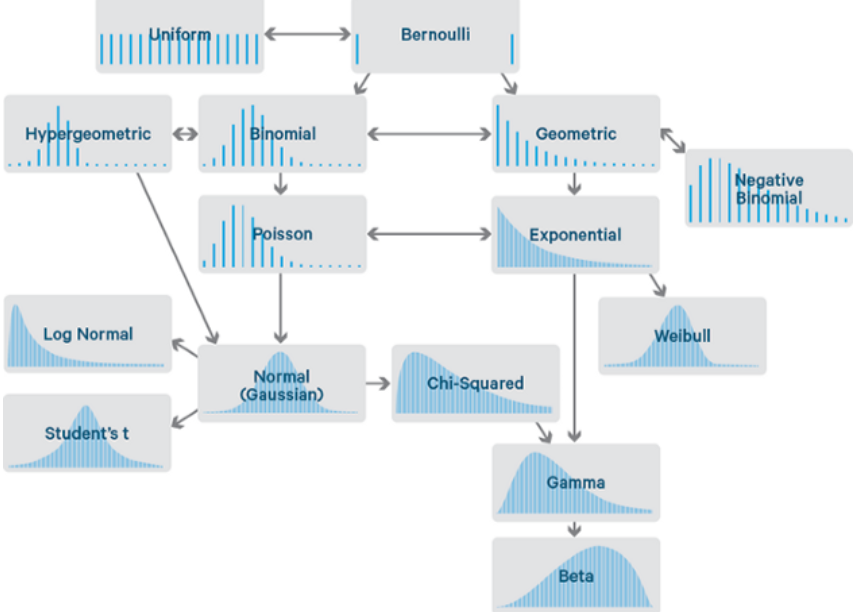
\includegraphics[scale=.4]{Distributions}
			\end{figure}
		\end{column}
		\begin{column}{0.3\paperwidth}
				\textbf{Discrete}
				\begin{enumerate}
					\item Uniform Discrete or Rectangular
					\setlength{\itemsep}{0.mm}
					\item Binomial
					\setlength{\itemsep}{0.mm}
					\item Hypergeometric
					\setlength{\itemsep}{0.mm}
					\item Poisson
					\setlength{\itemsep}{0.mm}
					\item Geometric
				\end{enumerate}
				\textbf{Continuous}
				\begin{enumerate}
					\item Uniform 
					\setlength{\itemsep}{0.mm}
					\item Normal/Gaussian
					\setlength{\itemsep}{0.mm}
					\item Student’s T
					\setlength{\itemsep}{0.mm}
					\item chi-squared
					\item Exponential
					\setlength{\itemsep}{0.mm}
					\item Beta
					\setlength{\itemsep}{0.mm}
					\item Triangular
					\setlength{\itemsep}{0.mm}
					\item Gamma

				\end{enumerate}
		
		\end{column}
	\end{columns}

\end{frame}






\begin{frame}
\begin{figure}
	\makebox[\linewidth]{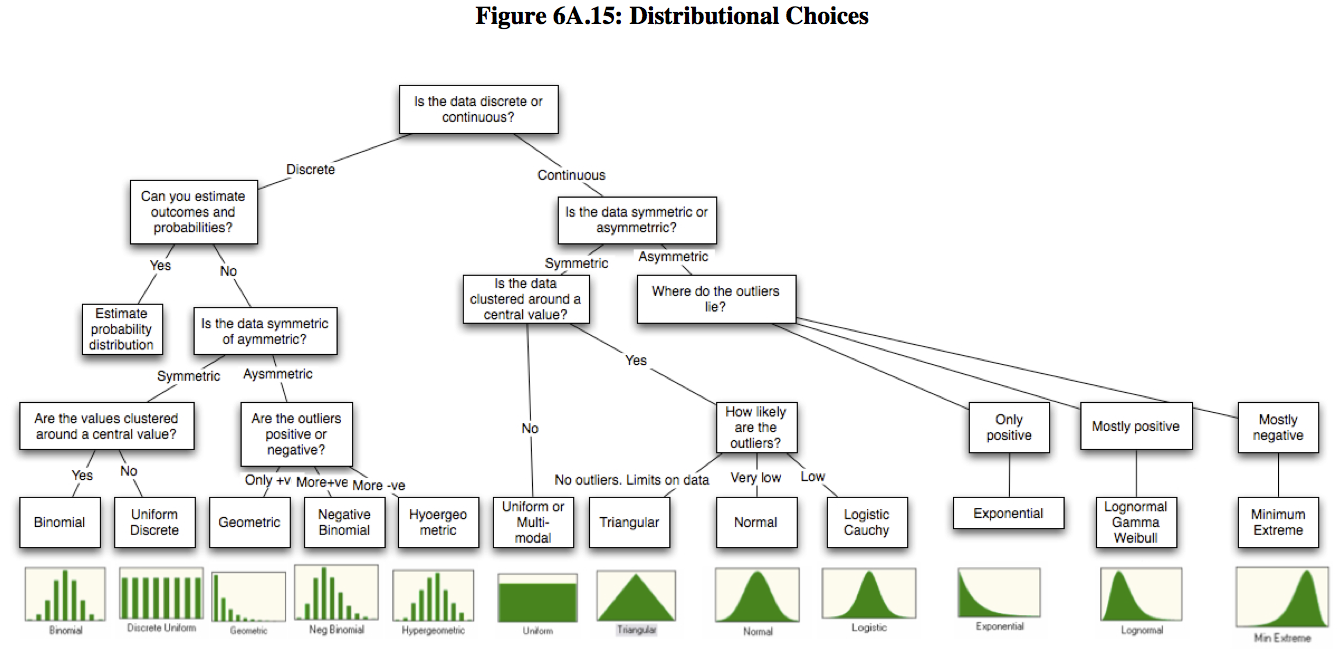
\includegraphics[width=\paperwidth]{distributionChoice}}
\end{figure}
\end{frame}


\begin{frame}[plain]\frametitle{}
	\makebox[\linewidth]{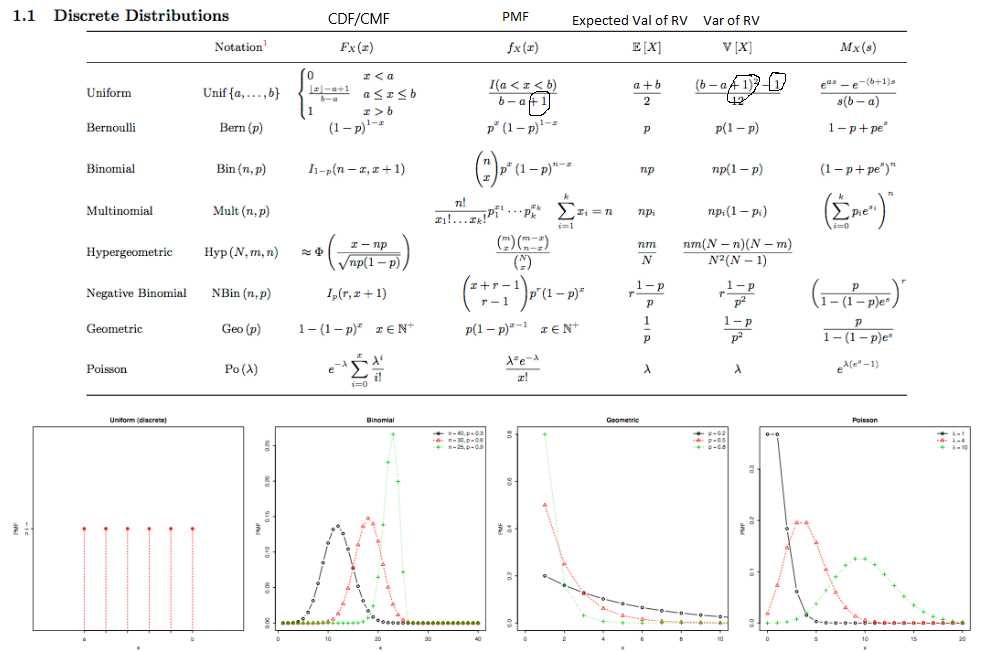
\includegraphics[width=\paperwidth]{DiscreteDistribution}}
\end{frame}


\begin{frame}
\begin{figure}
	\makebox[\linewidth]{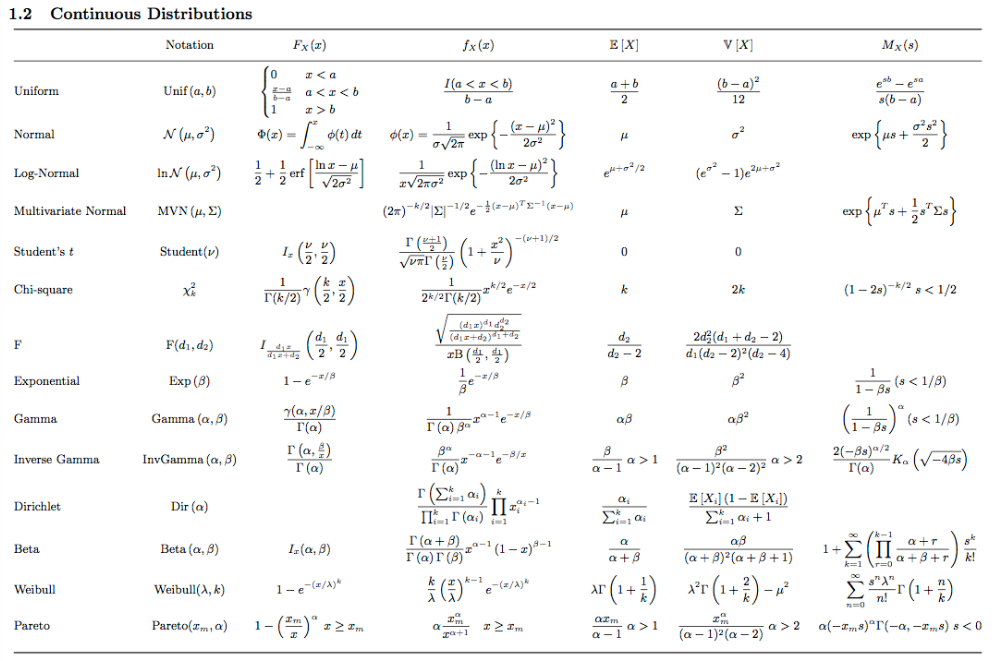
\includegraphics[width=\paperwidth]{ContinuousDistribution}}
\end{figure}
\end{frame}


\begin{frame}
\begin{figure}
	\makebox[\linewidth]{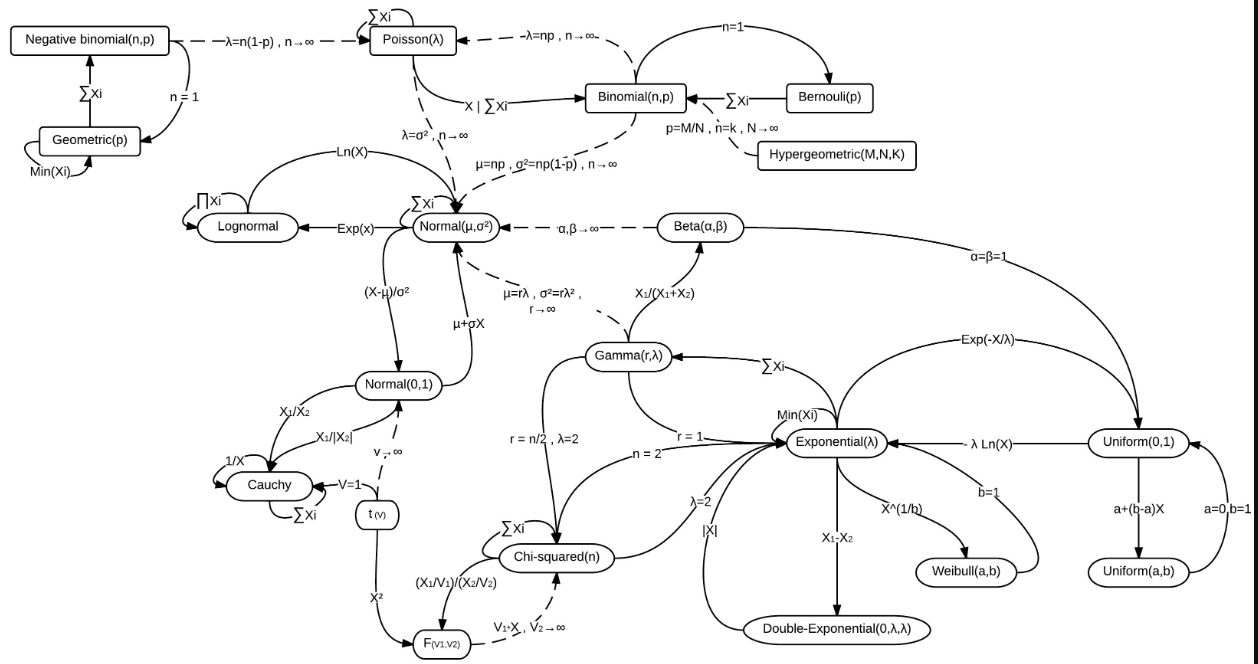
\includegraphics[width=\paperwidth]{UnivariateProbabDist}}
\end{figure}
\end{frame}







%%%%%%%%%%%%%%%%%%%%%%%%%%%%%%%%%%%%%%%%%%%%%%%%%%%%%%%%%%%%%%%

\begin{frame}\frametitle{relation btw various dist}
\textbf{Bernoulli and Binomial}: Bernoulli Distribution is a special case of Binomial Distribution with a single trial.

\textbf{Poisson and Binomial}: Poisson Distribution is a limiting case of binomial distribution under the following conditions:

The number of trials is indefinitely large or $\displaystyle{\lim_{x \to \infty}}$.
The probability of success for each trial is same and indefinitely small or $\displaystyle{\lim_{x \to 0}}$.
np = $\lambda$, is finite.

\textbf{Normal and Binomial}: Normal distribution is another limiting form of binomial distribution under the following conditions:

The number of trials is indefinitely large, $\displaystyle{\lim_{n \to \infty}}$.
Both p and q are not indefinitely small.
\textbf{Normal and Poisson Distribution}:
The normal distribution is also a limiting case of Poisson distribution with the parameter $\displaystyle{\lim_{\lambda \to \infty}}$.



\end{frame}

\begin{frame}{Beta and Binomial}
\textbf{Prior and Posterior}
\begin{enumerate}
\item 	Conjugate prior for binomial
$ x|p ~ Bin(n,p); p~Beta(a,b) [prior]$\\
$ f(p|X=k) = use bayes$ \\
$ replace with beta abd bin $ \\
$ p|X ~ Beta(a+X, b+n-x) $

\end{enumerate}
\end{frame}


\begin{frame}%\frametitle{Poisson va exponential}
\begin{columns}
\begin{column}{0.45\textwidth}
\textbf{Poisson}
event per unit time
\\how many calls do you get in a day
\\The number of printing errors at each page of the book
\\Num of metro arrivals in t time
\\The number of arrivals reported in an area on a day.
\\ The number of soldiers killed by horse-kick per year
\\ Air conditioners in a lifetime
\end{column}
\begin{column}{0.45\textwidth}
\textbf{exponential}
time per event
\\What about the interval of time btw the calls
\\Num of pages before until x num of printing errors
\\ Length of time btw metro arrivals,
\\ Length of time between arrivals at a gas station
\\Num of years btw horse-kick deaths in the army
\\ The life of an Air Conditioner

\end{column}

\end{columns}
\end{frame}




%%%%%%%%%%%%%%%%%%%%%%%%%%%%%%%%%%%%%%%%%%%%%%%%%%%%%%%%%%%%%%%%%%%%%%%%%%%%%%%%%%%%%%%%%%%%%%%%%%%%%%%%%%%%%%%%%%%%%%%%%%%%%%%%%%%%%%%%%%%%%%%%%%%%


\subsection{Distributions}
\begin{frame}\frametitle{Standard Uniform Density}
	parameters a = 0 and b = 1, so the PDF for standard uniform density is given by:
	
	\begin{align}
		f(x) = \left\{ \begin{array}{cc} 
		1, & \hspace{5mm} 0 <= x <=1 \\
		0, & \hspace{5mm} otherwise \\
		%T( \lfloor \frac{n}{2} \rfloor) + T(\lceil \frac{n}{2} \rceil)+ 2 & \hspace{5mm} n > 2 \\	
		\end{array} \right.
	\end{align}
	
\end{frame}


\begin{frame}\frametitle{Normal Distribution}
\textbf{Standard Normal Distribution} $\mu$ = 0 ; $\sigma$ = 1 \\
\textbf{The 68-95-99.7 rule}: Given a normally distributed random variable:
$P(\mu-\sigma \leq X \leq \mu+\sigma) \approx .68 =>$68\% of samples fall within 1 SD of the mean \\
$P(\mu-2\sigma \leq X \leq \mu+2\sigma) \approx .95$ \\
$P(\mu-3\sigma \leq X \leq \mu+3\sigma) \approx .997$ \\

characteristics of Normal distribution:
	\begin{enumerate}
		\item Mean = median = mode
		\item The distribution curve is bell-shaped and symmetrical about the line x=$\mu$.
		\item The total AUC = 1.
		\item Exactly half of the values are to the left of the center and the other half to the right.
	\end{enumerate}
	
\end{frame}

\begin{frame}\frametitle{Student's t distribution}
	characteristics\\
	\begin{enumerate}
		\item Underlying dist is Normal
		\item Pop dist is unknown
		\item sample size is too small for CLT to apply
	\end{enumerate}
	$z \sim \frac{\bar{x}-\mu}{\sigma/\sqrt{n}} \longleftrightarrow$
	$t_{n-1} \sim \frac{\bar{x}-\mu}{s/\sqrt{n}} $	
	\textbf{t test measures}
	\begin{enumerate}
		\item to test hypothesized population mean $\frac{\bar{x}-\mu}{s/\sqrt{n}}$
		\item regression $\frac{b-\beta}{SE(b)}$ (uses Std error, as pop std dev is known)
		\item 2 sampled t-test: assessing the diff btw 2 pop 
		$\frac{(\bar{x_1}-\mu_1)-(\bar{x_2}-\mu_2)}
		{\sqrt{\frac{s_1^2}{\sqrt{n_1}}+\frac{s_1^2}{\sqrt{n_1}}}}$
	\end{enumerate}
\end{frame}

\begin{frame}\frametitle{Chi-squared dist}
	comes directly from a normal dist (square of selection from standard Normal Distribution) so sample size should be large enough ($>$5) s.t. CLT applies\\
	for k degrees of freedom: $\chi_k^2 = \sum_{i=1}^{k}Z_i^2$\\
	$\chi = \sum\frac{(obs-exp)^2}{exp}$ with
	DF = (row-1)(col-1)\\
	\begin{figure}
		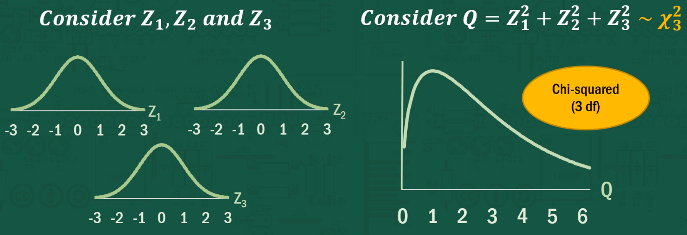
\includegraphics[scale=0.5]{chisq}
	\end{figure}
\end{frame}



\begin{frame}\frametitle{Binomial, bernoulli, hyper-geometric}
	Repeat Bernoulli n times and it's Binomial.\\
	Hypergeometric is Binomial without replacement\\

	the properties of a Binomial Distribution are
	\begin{enumerate}
		\item Each trial is independent.
		\item There are only two possible outcomes per trial.
		\item A total number of n identical trials are conducted.
		\item The probability of success and failure is same for all trials. (Trials are identical.)
	\end{enumerate}

\end{frame}


\begin{frame}\frametitle{Hypergeometric}
\begin{enumerate}
	\item Discrete
	\item equivalent to Binomial, without replacement
	\item N = total population\\ m=total items of interest in population\\n=sample size
	\item region bounded by 0 and m
\end{enumerate}
Characteristics of Poisson distribution:
\begin{enumerate}
	\item Event are not Independent.
	\item 
\end{enumerate}	

\end{frame}

\begin{frame}\frametitle{Poisson}
	\begin{enumerate}
		\item Discrete
		\item events in fixed region of opportunity (or time interval, t)
		\item region bounded by 0 and $\infty$
	\end{enumerate}
	Characteristics of Poisson distribution:
	\begin{enumerate}
		\item Independent event.
		\item The probability of success over a short interval must equal the probability of success over a longer interval.
		\item The probability of success in an interval approaches zero as the interval becomes smaller.
		\item The rate at which event occurs is constant ($\lambda$)
	\end{enumerate}	

	Poisson RV, $X$ = number of events in t.\\
	mean number of events in t, $\mu$ = $\lambda$*t\\
	The PMF of X: 	$P(X=x)=e^{-\mu}*\frac{\mu^x}{x!}$
\end{frame}


\begin{frame}\frametitle{Exponential Dist}
	inverse of Poisson: rate parameter or mean for poisson = $\lambda$ and mean for expo = $\beta=1/\lambda$ \\
	Exponential distribution is widely used for survival analysis.\\
	Memoryless-ness:\\
	events must occur at constant rate\\
	events must be independent of each other\\
	probab of event occurring in first min = probab of the event occuring in (t+1)min\\
	probab of first visitor on website in first min = p\\
	probab of first visitor on website in second min = (1-p)p\\
	probab of first visitor on website within third min = (1-p)$^2$p\\
	Each minute graph dropping $\rightarrow$ exponential decay
	

\end{frame}


\begin{frame}\frametitle{Memorylessness}
		Memoryless property: $P(X>=s+t | X>=s) = P(X>=t) $ \\
	$P(X>=s) = 1-CDF = 1-P(X<=s) = e^{-\lambda s}$ \\
	$P(X>=s+t | X>=s) = \frac{P(X>=s+t, X>=s)}{P(X>=s)}$ \\
	$P(X>=s+t | X>=s) = \frac{P(X>=s+t)}{P(X>=s)}$ \\
	$P(X>=s+t | X>=s) = \frac{e^{-\lambda (s+t)}}{ e^{-\lambda s}}$ \\
	$P(X>=s+t | X>=s) = e^{-\lambda t}$ \\
	Memoryless property: \\
	$E(X|X>a) = a+E(X-a|X>a)$ \\
	$E(X|X>a) = a+ 1/\lambda$ \\
	
\end{frame}


\begin{frame}%\frametitle{Poisson}
	\begin{columns}
		\begin{column}{0.45\textwidth}
			failure rate of any device at time t, given that it has survived up to t; $\lambda = \frac{1}{\beta} > 0 $
			\\ 
			\textbf{area under the density curve}
		\end{column}
		\begin{column}{0.5\textwidth}
			\begin{figure}
				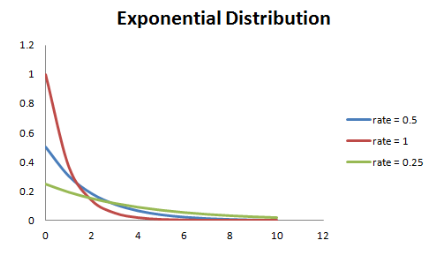
\includegraphics[scale=0.5]{exponential}
			\end{figure}
		\end{column}
	\end{columns}
			to the left of x
			 $P\{X \leq x\} = 1 – e^{-\lambda x}$
			\\ to the right of x $P\{X > x\} = e^{-\lambda x}$
			\\
			$P\{x1 < X \leq x2\} = e^{-\lambda x1} - e^{-\lambda x2}$

\end{frame}



\section{EDA}
\begin{frame}\frametitle{Univariate and Multivariate Analysis}
\end{frame}

\begin{frame}\frametitle{Dimensionality Reduction}
\end{frame}

\begin{frame}\frametitle{Under and Over Sampling}
\end{frame}


\section{Descriptive Statistics}



\begin{frame}%\frametitle{Variance, Standard Deviation} 
\begin{itemize}
	\item Variable and Random Variable (RV)
	\item Parameter and Hyper-parameter
	\item \hyperlink{meanlabel}{\beamerbutton{Mean}}, Median, Mode
	\item mode sucks for small samples
	\item Range, IQR
	\item Standard Deviation ($\sigma$): Measure of the how spread out data is from its mean.
	\item Variance ($\sigma^2$): It describes how much a random variable differs from its expected value. It entails computing squares of deviations.The average of the squared differences from the Mean.\\
	\begin{enumerate}
		\item Deviation is the difference bw each element from the mean.\\
		\item Population Variance = avg of squared deviations\\
		\item Sample Variance = avg of squared differences from the mean
	\end{enumerate}
\end{itemize}
\end{frame}

\begin{frame}
\hypertarget{meanlabel}{EXPECTED VALUE}\newline
\textbf{Discrete random variable}	$E(X) = \sum_x x \, p_x(x)$
\begin{itemize}
\item Provided $\sum_x |x| \, p_x(x) < \infty$. If the sum diverges, the expected value does not exist. 
\textbf{For the jar full of numbered balls}
\item A ball is selected at random; all balls are equally likely to be chosen $P(X = x_i) = \frac{1}{N}$.
\item Say $n_1$ balls have value $v_1$, and $n_2$ balls have value $v_2$, and \ldots  $n_n$ balls have value $v_n$. Unique values are $v_i$, for $i=1, \ldots, n$. Note $n_1 + \cdots + n_n = N$, and $P(X=v_j) = \frac{n_j}{N}$. 
$E(X) = \frac{\sum_{i=1}^N x_i}{N}$

\end{itemize}

\textbf{Continuous random variable}  $E(X) = \int_{-\infty}^\infty x \, f_x(x) \, dx$

\begin{itemize}
\item Provided $ \int_{-\infty}^\infty |x| \, f_x(x) \, dx < \infty$. If the integral diverges, the expected value does not exist. 

\end{itemize}

\end{frame}

%%%%%%%%%%%%%%%%%%%%%%%%%%%%%%%%%%%%%%%%%%%%%%%%%%%%%%%%%%%%%%%%%%%%%%%%%%%%%%%%%%%%%%%%%


\begin{frame}
\frametitle{Sometimes the expected value does not exist}
\framesubtitle{Need $ \int_{-\infty}^\infty |x| \, f_x(x) \, dx < \infty$}  
For the Cauchy distribution, $f(x) = \frac{1}{\pi(1+x^2)}$.  
\begin{eqnarray*}
E(|X|) & = & \int_{-\infty}^\infty |x| \, \frac{1}{\pi(1+x^2)} \, dx \\ 
& = & 2 \int_0^\infty \frac{x}{\pi(1+x^2)} \, dx \\ 
&& u = 1+x^2, ~du = 2x \, dx \\  
& = & \frac{1}{\pi} \int_1^\infty \frac{1}{u} \, du \\ 
& = & \ln u |_1^\infty \\ 
& = & \infty - 0 = \infty 
\end{eqnarray*} 
$=>$ an integral ``equals" infinity, it is unbounded above.
\end{frame}

%%%%%%%%%%%%%%%%%%%%%%%%%%%%%%%%%%%%%%%%%%%%%%%%%%%%%%%%%%%%%%%%%%%%%%%%%%%%%%%%%%%%%%%%%

\begin{frame}

For a RV $X$ with PDF $\rho(x)$. The variance($\mathbb{V}$) and the standard deviation($\sigma_X$) of $X$, are defined by

Variance   $\sigma^2 = (1/n)\sum_{i=1}^{n}(x_i - \mu)^2$

\begin{align*} \mathbb{V} &= \mathbb{E}\left[ \left( X-\mathbb{E}[X] \right)^2 \right]
=\mathbb{E}[X^2] - \mathbb{E}[X]^2
= \int_D (x-\mathbb{E})^2 \, dP. \end{align*}

\begin{align*} \mathbb{V} &= \int_D x^2 \, dP - \mathbb{E}^2. \end{align*} 

\begin{align*}\sigma_X&=\sqrt{V[X]}
&=\sqrt{E[X^2]-E[X]^2}
\end{align*}

\begin{align*} \mathbb{V} &=\sqrt{\int_D x^2\rho(x)\,dx - \left(\int_D x\rho(x) \,dx\right)^2}. \end{align*}


\end{frame}


\begin{frame}
If one interprets the PDF ($\rho(x)$) as the density of a rod at location ($x$), then:\\

The mean, ($\mu = \int x\rho(x)\,dx$), gives the center of mass of the rod.\\
The variance, ($V = \int (x-\mu)^2\rho(x)\,dx$), gives the moment of inertia about the line ($x = \mu$).\\
The standard deviation, ($\sigma = \sqrt{V}$), gives the radius of gyration about the line ($x = \mu$).

\end{frame}

\begin{frame}\frametitle{Std error vs std deviation}
std error = 
\end{frame}


\begin{frame}\frametitle{coeff of variation}
$CV = \frac{sd}{\bar{x}}, where  \bar{x}=sample mean$ \\
$x = [1,2,3] => \bar{x}=2$ and $S_x=1 => CV(x)=1/2 $\\
$y = [101,102,103] => \bar{y}=102$ and $S_y=1 => CV(y)=1/102 $\\
Higher the CV means higher fluctuations in the dataset\\

\end{frame}


\begin{frame}\frametitle{skewness and kurtosis}
\textbf{skewness}\\
mode skewness = $\frac{mean-mode}{std dev}$\\
in skewed data: mode = 3(median) - 2(mean) \\
for small dataset, use below:\\
median skewness = $\frac{3(mean-median)}{std dev}$\\
\begin{align}
skewness = \left\{ \begin{array}{cc} 
approx\_symmetric, & \hspace{5mm} -0.5 <= x <=0.5 \\
moderately\_skewed, & \hspace{5mm} 0.5< |x| <1 \\
highly\_skewed, & \hspace{5mm} |x|>1 \\
\end{array} \right.
\end{align}
\textbf{kurtosis}: same mean or sd but diff peakedness\\
higher peaked $=>$ higher kurtosis \\	

\end{frame}

\begin{frame}\frametitle{Moments}
\textbf{I moment}: $\frac{\sum x}{n} =>$ \textbf{mean} $=>$ considered as values from 0\\
second moment: $\frac{\sum x^2}{n} => $values further from 0 will be higher, \\so instead we take centralized \\
second (centralized) moment: $\frac{\sum (x-\mu)^2}{n} =>$ variance\\
third (centralized) moment: $\frac{1}{n} \frac{\sum (x-\mu)^3}{\sigma ^3} ->$ skew\\
but since we don't have population mean, we have sample mean, we adjust the above value with degrees of freedom\\
\textbf{II (centralized) moment}: $\frac{\sum (x-\bar{x})^2}{n-1} =>$ \textbf{variance}\\
\textbf{III (centralized) moment}: $\frac{n}{(n-1)(n-2)} \frac{\sum (x-\bar{x})^3}{s^3} =>$ \textbf{skew}\\
\textbf{IV moment}: $\frac{n(n+1)}{(n-1)(n-2)(n-3)} \frac{\sum (x-\bar{x})^4}{s^4}-\frac{3(n-1)^2}{(n-2)(n-3)} =>$ \textbf{kurtosis}\\

\end{frame}


%%%%%%%%%%%%%%%%%%%%%%%%%%%%%%%%%%%%%%%%%%%%%%%%%%%%%%%%%%%%%%%%%%%%%%%%%%%%%%%%%%%%%%%%%

\section{Experimental Design}

\subsection{Hypothesis testing}

\begin{frame}\frametitle{p\_value}
p-value is the probab of getting a sample as extreme as ours, given $H_0$ is true\\
when population std dev is known then we use z-statistics, if unknown then we use t-statistics\\
t-statistics assumes that underlying distribution is normal\\
t-distribution is bell curved, defined by it's DF (degrees of freedom)\\

\end{frame}


\begin{frame}[plain]
\begin{columns}
	\begin{column}{0.72\textwidth}
		\begin{figure}
			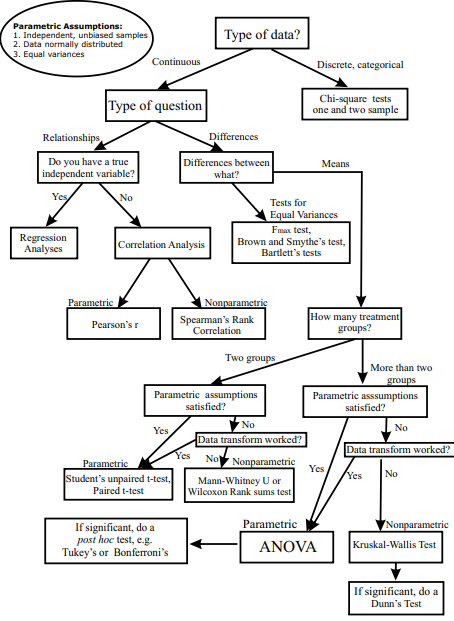
\includegraphics[scale=0.54]{statisticaltest}
		\end{figure}
	\end{column}
	\begin{column}{0.3\textwidth}
		\begin{enumerate}
			\item $H_0: \mu=100$; $H_1: \mu \ne 100$
			\item if $H_0$ is true, how extreme is our sample?
			\item Measure of extremeness, z=$\frac{\bar{x}-\mu}{\sigma/\sqrt{n}}$
			\item $\uparrow$ z value, more likely to reject $H_0$
			\item either reject $H_0$ or do not reject $H_0$ because there's less evidence to reject it (given $\alpha$ level of significance)
		\end{enumerate}
	\end{column}
\end{columns}
\end{frame}


{%<--- Start local changes
	\setbeamertemplate{navigation symbols}{}
	\usebackgroundtemplate{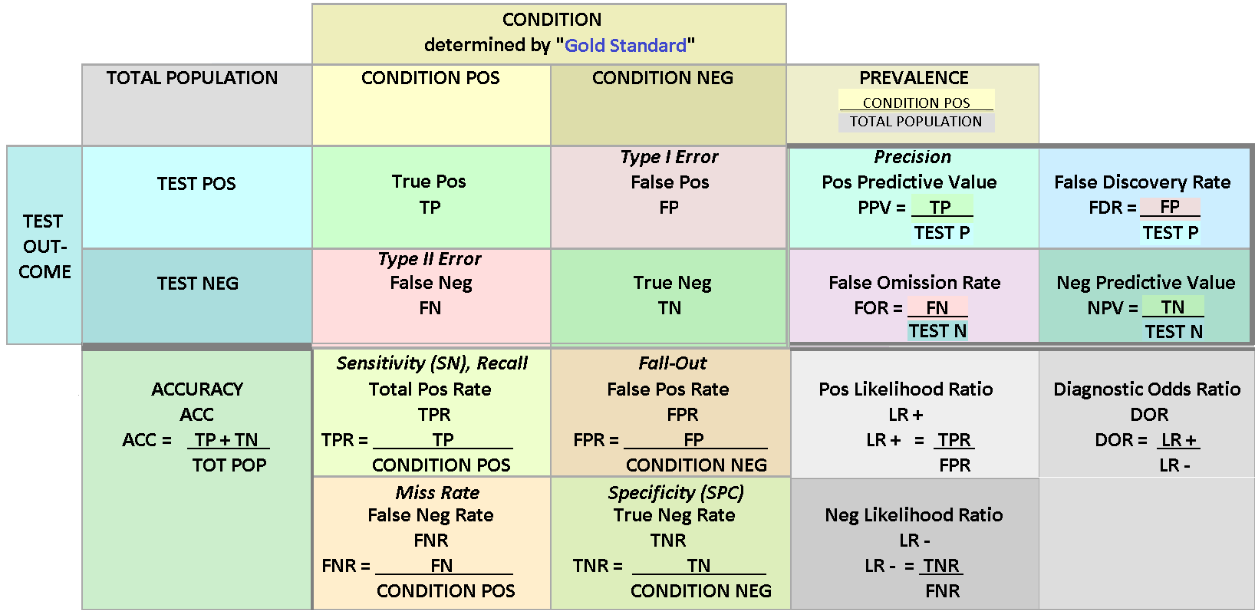
\includegraphics[width=\paperwidth]{confusionmatrix}}
	\begin{frame}[plain]
	\vspace{2.5in}
	\textbf{Type I Error}: Reject $H_0$ when $H_0$ is true \\
	Prob of Type I Error = level of significance = $\alpha$  5\% (generally)\\
	\textbf{Type II error}: Not reject $H_0$ when $H_0$ is false \\
	Prob of Type II Error = $\beta$ and power of hypothesis test = 1-$\beta$ \\
	1-$\beta$ = prob of rejecting a $H_0$ when $H_0$ is false\\
	%actual pos $=> H_1 is true$ test outcome is neg $=>$
	
	\end{frame}
}%<---- Finish local changes




\begin{frame}%[plain]
\begin{figure}\frametitle{test statistics}
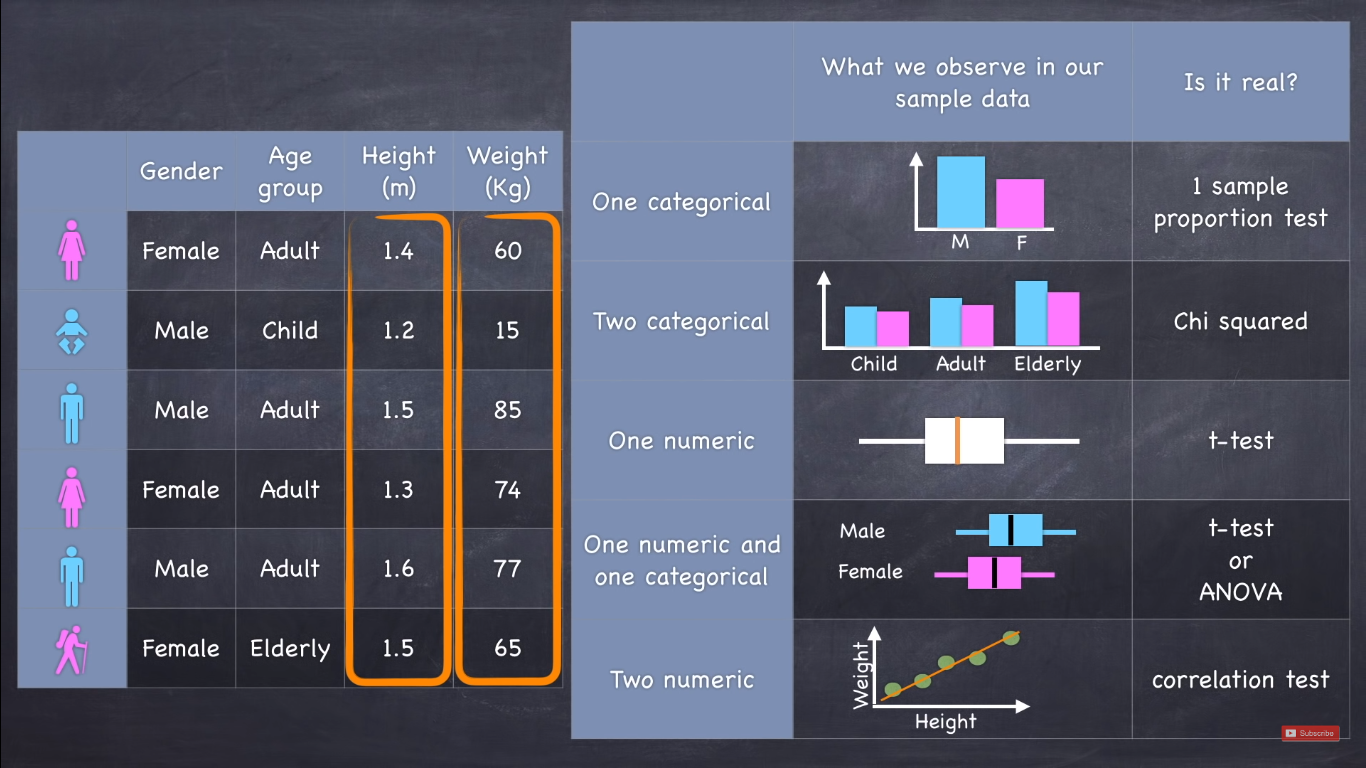
\includegraphics[scale=0.28]{TypesTests} 
\caption{t-test, anova, chi-square, correlation test}
\end{figure}
\end{frame}



\begin{frame}[plain]
\makebox[\linewidth]{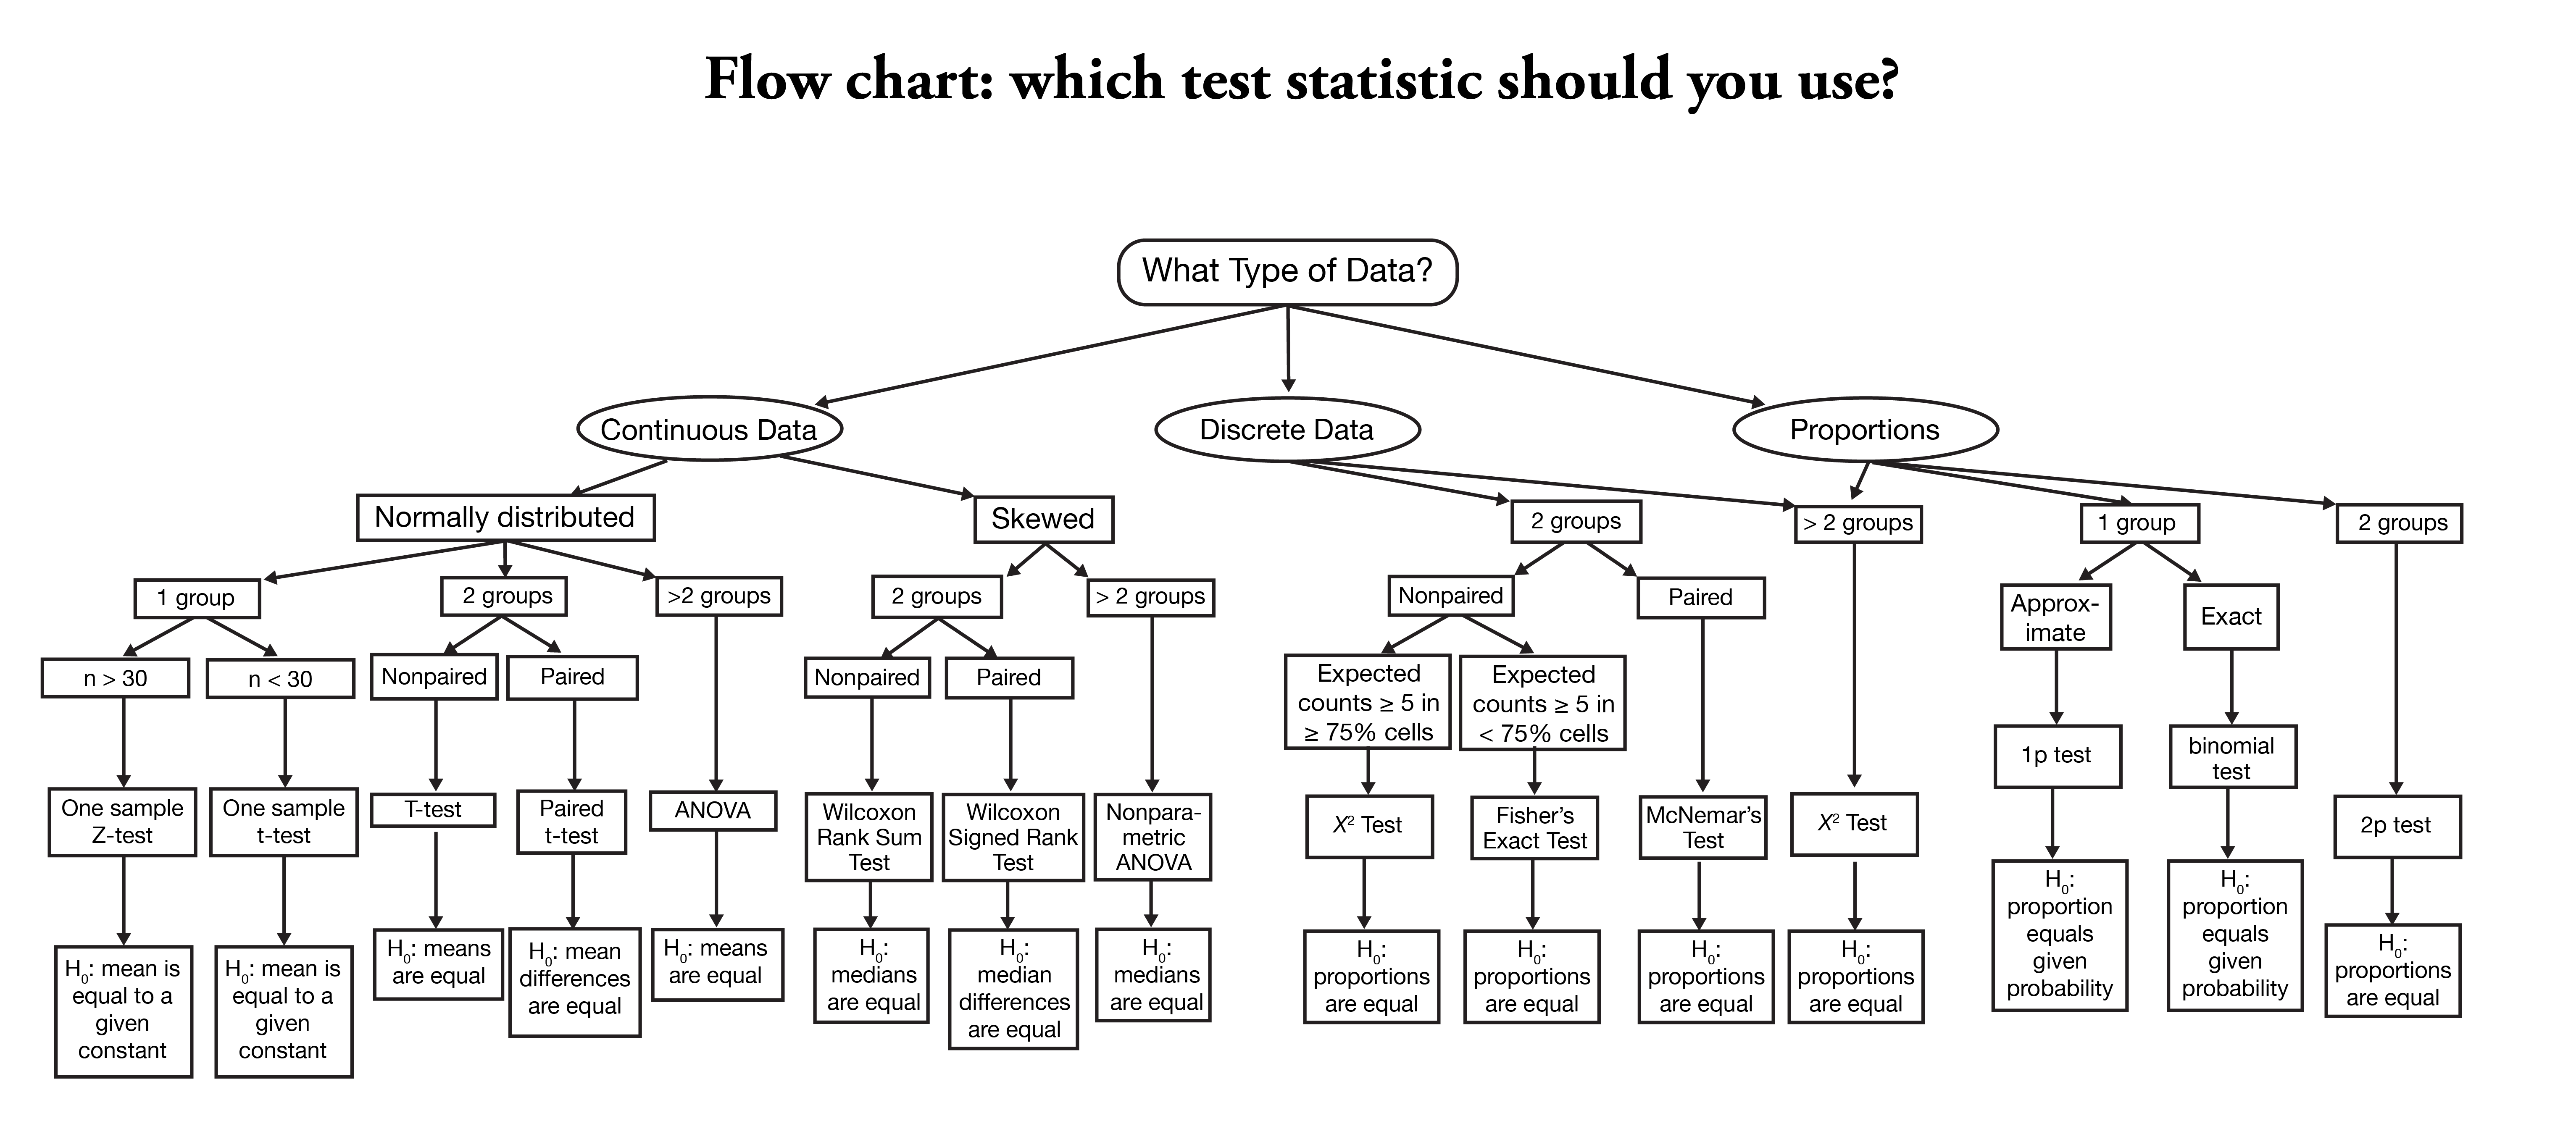
\includegraphics[width=\paperwidth]{teststats}}
\end{frame}

\begin{frame}\frametitle{When can AB test fail}
	\begin{enumerate}
		\item in the case of a \textbf{referral program}, The referrer and Referee could be split across test and control groups causing spillover on the control or variant group
		\item Novelty effects: Prompts and CTA tend to exhibit novelty effects, if not measuring their performance over the long term using a holdout a wrong attribution and/or customer fatigue can happen.
		\item What-if scenarios: If you are looking to understand the impact of \textbf{not having launched a product}, for instance a subscription offering on a website. A/B test wouldn’t be the right fit.
	\end{enumerate}
\end{frame}


\begin{frame}
	Class Imbalance
\end{frame}


%%%%%%%%%%%%%%%%%%%%%%%%%%%%%%%%%%%%%%%%%%%%%%%%%%%%%%%%%%%%%%%%%%%%%%%%%%%%%%%%%%%%%%%


\section{Bayesian Statistics}

\subsection{blocs}
\begin{frame}\frametitle{blocs}

\begin{block}{title of the bloc}
bloc text
\end{block}

\begin{exampleblock}{title of the bloc}
bloc text
\end{exampleblock}


\begin{alertblock}{title of the bloc}
bloc text
\end{alertblock}
\end{frame}



\begin{frame}
	MACHINE LEARNING
	
	chi square
	
	big O notation
	
	
	book - kevin murphy
	
	Precision Recall tradeoff
	How to choose the method of predictive modelling.
	algorithms
	Bayesian Modelling (Topic Modelling), NLP, Bayesian Nonparametric Techniques, Social Network Analysis, Sentiment Analysis
	- https://www.springboard.com/blog/machine-learning-interview-questions/
	- https://www.quora.com/What-is-the-difference-between-supervised-and-unsupervised-learning-algorithms
	
	https://blog.udacity.com/2016/04/5-skills-you-need-to-become-a-machine-learning-engineer.html
	https://towardsdatascience.com/how-to-build-a-data-science-portfolio-5f566517c79c
	
	http://www.smdi.com/evolution-machine-learning
	https://vinodsblog.com/2018/03/11/the-exciting-evolution-of-machine-learning/
	
	
	https://software.intel.com/en-us/articles/an-introduction-to-neural-networks-with-an-application-to-games
	
	https://towardsdatascience.com/introduction-to-neural-networks-advantages-and-applications-96851bd1a207
	
	What are type 1 error and type 2 error? what is p-value 
	
	ML
	https://www.youtube.com/watch?v=qv6UVOQ0F44
	
	https://www.quora.com/What-is-the-relation-between-standard-normal-and-gamma-distribution
	
	
	https://stats.stackexchange.com/questions/37461/the-relationship-between-the-gamma-distribution-and-the-normal-distribution
	
	http://www.statisticshowto.com/probability-and-statistics/regression-analysis/
	(go to definitions)
	
	https://www.thoughtco.com/what-is-kurtosis-3126241
	
	http://www.statisticshowto.com/what-is-statistical-significance/
	
	https://en.wikipedia.org/wiki/F-test
	
	numpy matplotlib
	
	http://slideplayer.com/slide/6260251/
	
	http://www.sfu.ca/~ber1/iat802/pdfs/When%20to%20use%20what%20test.pdf
	
	https://www.youtube.com/watch?v=RlhnNbPZC0A
\end{frame}

%%%%%%%%%%%%%%%%%%%%%%%%%%%%%%%%%%%%%%%%%%%%%%%%%%%%%%%%%


\begin{frame}

\end{frame}

\begin{frame}
	Thank You!
\end{frame}

\end{document}